% Full instructions available at:
% https://github.com/elauksap/focus-beamertheme

\documentclass[9pt]{beamer}
\usetheme{focus}

%%%%%%%%%%%%%%%%%%%%%%%%%%%%%%%%%%%%%%%%%%%%%%%%%%%%%%%%%%%%%%%%%%%%%
% Typography, change document font
\usepackage[tt=false, type1=true]{libertine}
\usepackage[varqu]{zi4}
\usepackage[libertine]{newtxmath}
\usepackage[T1]{fontenc}

\usepackage[protrusion=true,expansion=true]{microtype}

% Disable paragraph indentation, and increase gap
\usepackage{parskip}

%Matrix
\usepackage{tabstackengine}
\setstackEOL{;}% row separator
\setstackTAB{,}% column separator
\setstacktabbedgap{1ex}% inter-column gap 
\setstackgap{L}{1.0\normalbaselineskip}% inter-row baselineskip
\let\mat\bracketMatrixstack

\newcommand{\pth}{Figure/}
\newcommand{\ve}[1]{\mathbf{#1}}

% Copyright (C) 2018-2019 Pasquale Claudio Africa and the LaTeX community.
% A full list of contributors can be found at
%
%     https://github.com/elauksap/focus-beamertheme
% 
% This file is part of beamerthemefocus.
% 
% beamerthemefocus is free software: you can redistribute it and/or modify
% it under the terms of the GNU General Public License as published by
% the Free Software Foundation, either version 3 of the License, or
% (at your option) any later version.
% 
% beamerthemefocus is distributed in the hope that it will be useful,
% but WITHOUT ANY WARRANTY; without even the implied warranty of
% MERCHANTABILITY or FITNESS FOR A PARTICULAR PURPOSE. See the
% GNU General Public License for more details.
% 
% You should have received a copy of the GNU General Public License
% along with beamerthemefocus. If not, see <http://www.gnu.org/licenses/>.

\mode<presentation>


% DEFINE COLORS. ---------------------------------------------------------------
\definecolor{main}{RGB}{134, 161, 174}
\definecolor{main2}{RGB}{104, 131, 144}
\definecolor{textc}{RGB}{20, 20, 20}
\definecolor{background}{RGB}{255, 255, 255}

\definecolor{alert}{RGB}{180, 0, 0}
\definecolor{example}{RGB}{0, 110, 0}


% SET COLORS. ------------------------------------------------------------------
\setbeamercolor{normal text}{fg=textc, bg=background}
\setbeamercolor{alerted text}{fg=textc}
\setbeamercolor{example text}{fg=textc}

\setbeamercolor{titlelike}{fg=background, bg=main}
\setbeamercolor{frametitle}{parent={titlelike}}

\setbeamercolor{footline}{fg=background, bg=main2}

\setbeamercolor{block title}{bg=main!80!background, fg=background}
\setbeamercolor{block body}{bg=main!10!background, fg=textc}

\setbeamercolor{block title alerted}{bg=alert, fg=background}
\setbeamercolor{block body alerted}{bg=alert!10!background, fg=textc}

\setbeamercolor{block title example}{bg=example, fg=background}
\setbeamercolor{block body example}{bg=example!10!background, fg=textc}

\setbeamercolor{itemize item}{fg=textc}
\setbeamercolor{itemize subitem}{fg=textc}

\setbeamercolor{enumerate item}{fg=textc!70!black}
\setbeamercolor{enumerate subitem}{fg=textc!70!black}

\setbeamercolor{description item}{fg=textc!70!black}
\setbeamercolor{description subitem}{fg=textc!70!black}

\setbeamercolor{caption name}{fg=textc}

\setbeamercolor{section in toc}{fg=textc}
\setbeamercolor{subsection in toc}{fg=textc}
\setbeamercolor{section number projected}{bg=textc}
\setbeamercolor{subsection number projected}{bg=textc}

\setbeamercolor{bibliography item}{fg=main}
\setbeamercolor{bibliography entry author}{fg=main!70!black}
\setbeamercolor{bibliography entry title}{fg=main}
\setbeamercolor{bibliography entry location}{fg=main}
\setbeamercolor{bibliography entry note}{fg=main}

\mode<all>


\begin{document}
\tableofcontents

\section{Directional Derivative : \today}
	\begin{frame}{Directional derivative}
		\begin{itemize}
			\item The directional derivative basically states how a function changes along a certain direction
			\item We can use it to linearise a nonlinear function , which gives us our Newton Rhapson method
			\item Finding the changes of a functional \footnote{Function of functions} with respect to its corresponding functions. This is akin to the variational or virtual work theorems
			\item The directional derivative gives the linear change!!! So at a point in the domain, it gives the linear change (Gradients) in a certain direction
			
		\end{itemize}
	\end{frame}


	\begin{frame}
		\begin{figure}
			\centering
			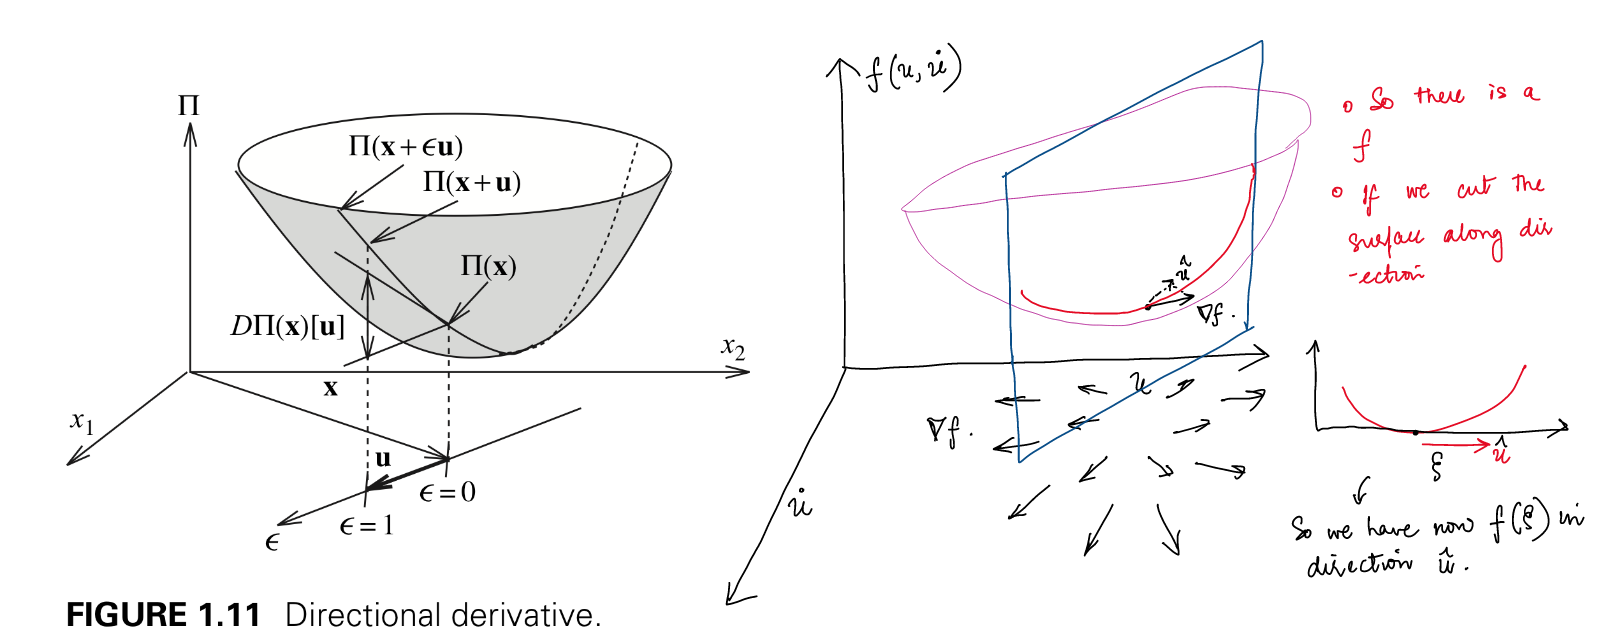
\includegraphics[width=1\linewidth]{Figure/fig1}
			\label{fig:fig3}
		\end{figure}
		\begin{itemize}
			\item So we have a funcitonal which depends on differerent functions or $\ve{x}$
			\item We cut the function with a plane (Blue) which gives us a curve how the function changes along that direction
			\item Finding that linear change along the direction ${u}$ \footnote{Remember that $u$ is a unit vector} gives the directional derivative. See that the curve is now dependant on $\epsilon$
			
			\item It is denoted as $\nabla_u$ or $D f(\ve{x})[u]$
			
		\end{itemize}
	\end{frame}

	\begin{frame}{Example \#1}
		\begin{figure}
			\centering
			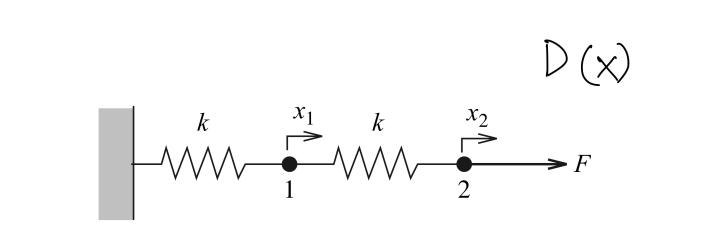
\includegraphics[width=0.5\linewidth]{Figure/fig2}
			\label{fig:fig2}
		\end{figure}
		\begin{itemize}
			\item Potential energy of the structure is
			\begin{align*}
				f(\ve{x}) = \frac{1}{2}kx_1^2 + \frac{1}{2}k(x_2-x_1)^2 - Fx_2 \\
				f(\ve{x+u}) = \frac{1}{2}k(x_1+u_1)^2 + \frac{1}{2}k(x_2 + u_2-x_1-u_1)^2 - F(x_2 + u_2) \\ 
				Df(\ve{x})[\ve{u}] \approx f(\ve{x+u}) - f(\ve{x}) 			
			\end{align*}	
			\item  Its approx $\approx$ as we want only the linear change, this is also what we mean when we write $\delta$f in variational calculus		
		\end{itemize}
	\end{frame}

	\begin{frame}
		\begin{itemize}
			\item How do we get the linear function? Taylor series!
			\begin{align*}
			f(\ve{x+\epsilon u}) = \frac{1}{2}k(x_1+\epsilon u_1)^2 + \frac{1}{2}k(x_2 + \epsilon u_2-x_1-\epsilon u_1)^2 - F(x_2 + \epsilon u_2) \\ 
			Df(\ve{x})[\ve{u}] \approx f(\ve{x+u}) - f(\ve{x}) \left(\text{Approx as only the linear change} \right)			
			\end{align*}
			\item This is the function on the plane that cuts the surface given in terms of $\epsilon$
			\item Linearise it about the point we get (And ignoring higher order terms)
			\begin{align*}
				f(\ve{x+\epsilon u}) = f(\ve{x}) + \left(\frac{ d}{ d\epsilon}|_{\epsilon = 0} f(\ve{x+\epsilon u}) \right) \epsilon + O(\epsilon^2)
			\end{align*}
			\item So our potential energy becomes , Take $\epsilon =1$ for unit direction
			\begin{align*}
			Df(\ve{x})[\ve{u}] = \left(\frac{ d}{ d\epsilon}|_{\epsilon = 0} f(\ve{x+\epsilon u}) \right) \\
			= \frac{ d}{ d\epsilon}|_{\epsilon = 0}\left(  \frac{1}{2}k(x_1+\epsilon u_1)^2 + \frac{1}{2}k(x_2 + \epsilon u_2-x_1-\epsilon u_1)^2 - F(x_2 + \epsilon u_2) \right) \\
			=k_1x_1u_1 + k(x_2-x_1)(u_2-u_1) - Fu_2 \\
			= \ve{u^T(Kx-F)}
			\end{align*}
		\end{itemize}
	\end{frame}

	\begin{frame}{Insight}
		\begin{itemize}
			\item So we get the form $\ve{u^T(Kx-F)}$ for some direction $\vec{u}$
			\item Equilbrium is satisfied when the potential is minimum for any $\vec{u}$ So $Df(x)[u] =0$
			\item This is exactly like the variational principle where we get something like $Df(x)[\delta u] =0$
			\item Where the Equilibrium has to be zero  $\ve{(Kx-F)}$ and therefore any work done on it by any displacment is zero ("Virtual displcament theory")
			\item At equilibrium the work done by the external and internal loads is equal to zero
			\item The functional may be still nonlinear with respect to $\ve{x}$ but we are linearising the function with respect to the change or direction $\ve{u}$ 
		\end{itemize}
	\end{frame}


	\section{Potential energy}
	\begin{frame}
		\begin{itemize}
			\item I have always had a confusion whether the potential energy is defined with respect to the position or with respect to displacements
			\item The answer is more nuanced. It can be with both but the times when it is used has to be understood properly in terms of what it actually represents.
			\item The Residual is the derivative of the potential energy with respect to its degrees of freedom
		\end{itemize}
	\end{frame}

	\begin{frame}
		\begin{equation}
			\Pi() = \text{Internal - External potential}
		\end{equation}
		Now suppose $\ve{x}$ is the position and $\ve{u}$ are the nodal dispalcements.
		Can write
		\begin{equation}
			\Pi(\ve{x}) = C(x_1 - x_2)  - Px_1 - Px_2
		\end{equation}
		where we say that C is a material parameter, and P are external loads. Now there is a problem with this equation because the internal energy is defined with respect to the relative displacements/deformation/displacement gradients of the continuum. 
		
		A more correct way is to write
		\begin{equation}
		\Pi(\ve{u}) = C(u_1 - u_2)  - Pu_1 - Pu_2
		\end{equation}
		So now the difference in the displacements gives the deformation that results in the strain energy. 
		
		However what about the external work. The external work can be thought of as the potential of the load due it's movement in u. It can also be sometimes thought of as the potential due to its' position, in the case of the well known potential of a ball = mgh, where h is it's position. But here the difference is P is dependant on h.
	\end{frame}

	\begin{frame}
		\begin{itemize}
			\item One way in which that can be made clear is if we represent the potential with respect to the position, but we include the initial undeformed position to give the displacement. It would look something like this:
			\begin{equation}
				\Pi(\ve{x}) = C((x_1  - x_{1ref})- (x_2- x_{2ref}) ) - P(x_1  - x_{1ref}) - P(x_2- x_{2ref})
			\end{equation}
			where the ref are the initial coordinates. So we can see that in the external work the coefficients $Px_{1ref}$ are constants and so are not important when you only want to minimize the potential energy. So Pu and Px are okay!
	 	\end{itemize}
	\end{frame}


	\begin{frame}
		 We can find the directional derivative of different things like the determinant of a matrix etc. Check Bonet Page 16
	\end{frame}

\end{document}